\documentclass[tikz,border=6pt]{standalone}
\usepackage[T1]{fontenc}
\usepackage[utf8]{inputenc}
\usepackage{pgfplots}
\usepgfplotslibrary{groupplots}
\usetikzlibrary{calc}
\pgfplotsset{compat=1.18}
\begin{document}
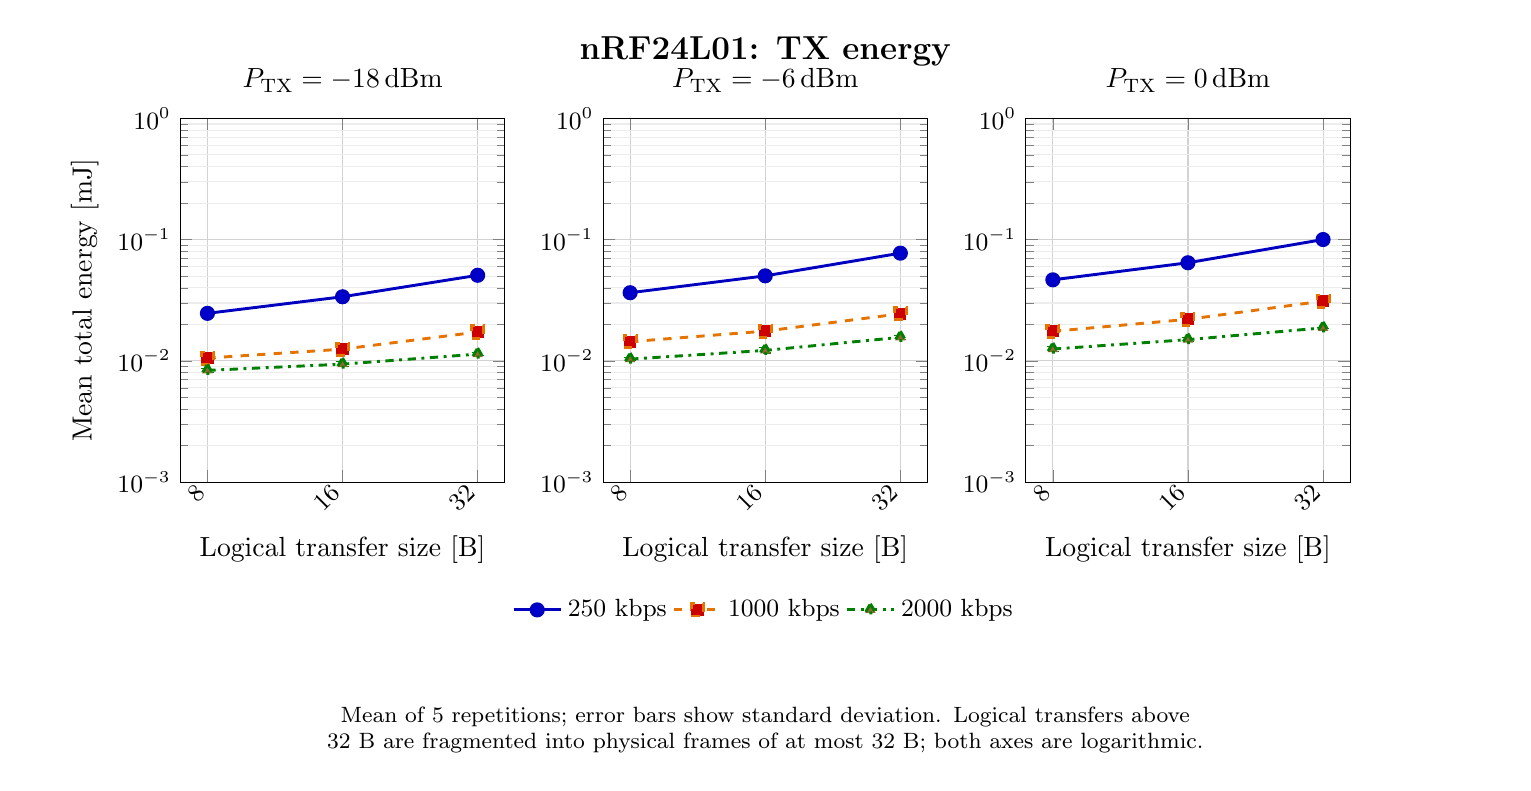
\begin{tikzpicture}
\begin{groupplot}[/pgf/number format/use comma,
  group style={group size=3 by 1, horizontal sep=1.25cm},
  width=5.7cm, height=6.2cm,
  xmode=log, log basis x={2}, ymode=log, log basis y={10},
  ymin=0.001, ymax=1,
  xtick={8,16,32}, xticklabels={8,16,32},
  x tick label style={rotate=45, anchor=east, font=\small},
  y tick label style={font=\small},
  grid=both, minor grid style={gray!15}, major grid style={gray!35},
  xlabel={Logical transfer size [B]},
  every axis plot/.append style={line width=1.05pt},
  error bars/error bar style={line width=0.35pt},
  legend style={font=\small, draw=none, fill=none, at={(0.5,-0.29)},
    anchor=north, legend columns=-1},
]
\nextgroupplot[title={\(P_{\mathrm{TX}}=-18\,\mathrm{dBm}\)}, ylabel={Mean total energy [mJ]}]
\addplot+[
  color=blue!75!black, solid, mark=*, mark size=2.2pt,
  error bars/.cd, y dir=both, y explicit,
] coordinates {
  (8,0.0246692408) +- (0,0.000581399284)
  (16,0.033805913) +- (0,0.000301893494)
  (32,0.05084354) +- (0,0.000553858953)
};
\addplot+[
  color=orange!90!black, dashed, mark=square*, mark size=2.2pt,
  error bars/.cd, y dir=both, y explicit,
] coordinates {
  (8,0.0105515359) +- (0,0.000442651096)
  (16,0.0124973133) +- (0,0.000413052043)
  (32,0.0173056222) +- (0,0.000202872062)
};
\addplot+[
  color=green!50!black, dashdotted, mark=triangle*, mark size=2.2pt,
  error bars/.cd, y dir=both, y explicit,
] coordinates {
  (8,0.0083475975) +- (0,0.000316828153)
  (16,0.00940235349) +- (0,0.000477725137)
  (32,0.0113711205) +- (0,0.000351284459)
};
\nextgroupplot[title={\(P_{\mathrm{TX}}=-6\,\mathrm{dBm}\)}]
\addplot+[
  color=blue!75!black, solid, mark=*, mark size=2.2pt,
  error bars/.cd, y dir=both, y explicit,
] coordinates {
  (8,0.0364990748) +- (0,0.000500347044)
  (16,0.0503017067) +- (0,0.000392545419)
  (32,0.0773781465) +- (0,0.000492389347)
};
\addlegendentry{250 kbps}
\addplot+[
  color=orange!90!black, dashed, mark=square*, mark size=2.2pt,
  error bars/.cd, y dir=both, y explicit,
] coordinates {
  (8,0.0143967425) +- (0,0.000416447298)
  (16,0.0176060151) +- (0,0.000382902591)
  (32,0.0244682162) +- (0,0.000412803697)
};
\addlegendentry{1000 kbps}
\addplot+[
  color=green!50!black, dashdotted, mark=triangle*, mark size=2.2pt,
  error bars/.cd, y dir=both, y explicit,
] coordinates {
  (8,0.0103433878) +- (0,0.000270366874)
  (16,0.0122048784) +- (0,0.000584374095)
  (32,0.0156478232) +- (0,0.000686445155)
};
\addlegendentry{2000 kbps}
\nextgroupplot[title={\(P_{\mathrm{TX}}=0\,\mathrm{dBm}\)}]
\addplot+[
  color=blue!75!black, solid, mark=*, mark size=2.2pt,
  error bars/.cd, y dir=both, y explicit,
] coordinates {
  (8,0.0466266501) +- (0,0.000324716118)
  (16,0.064486275) +- (0,0.000599202896)
  (32,0.100276659) +- (0,0.000371947873)
};
\addplot+[
  color=orange!90!black, dashed, mark=square*, mark size=2.2pt,
  error bars/.cd, y dir=both, y explicit,
] coordinates {
  (8,0.0175367568) +- (0,0.000241839598)
  (16,0.0220227424) +- (0,0.000386518792)
  (32,0.0311471279) +- (0,0.000264307783)
};
\addplot+[
  color=green!50!black, dashdotted, mark=triangle*, mark size=2.2pt,
  error bars/.cd, y dir=both, y explicit,
] coordinates {
  (8,0.0125237678) +- (0,0.00060204333)
  (16,0.0149738187) +- (0,0.000583839576)
  (32,0.0187308938) +- (0,0.000208975714)
};
\end{groupplot}
\node[font=\bfseries\large] at ($(group c2r1.north)+(0,0.85cm)$)
  {nRF24L01: TX energy};
\node[font=\footnotesize, align=center, text width=18.5cm]
  at ($(group c2r1.south)+(0,-3.15cm)$)
  {Mean of 5 repetitions; error bars show standard deviation. Logical transfers above 32 B are fragmented into physical frames of at most 32 B; both axes are logarithmic.};
\end{tikzpicture}
\end{document}
